\begin{graphicspathcontext}{{./chapters/simulation/examples/imgs/},{./chapters/simulation/examples/imgs/auto/},\old}

\begin{frame}{Carpooling Simulation Model}
	\begin{block}{For each day, for each individual}
		\begin{enumerate}
		\item Select the best transport mode according to the individual characteristics.
		\item Create a motive to carpool.
		\item Communicate this motive with other agents.
		\item Negotiate a plan with the interested agents.
		\item Execute the agreed plans.
		\item Provide a feedback to all concerned agents.
		\end{enumerate}
	\end{block}
	\vfill
	\cite{galland.abmtrans13}\hfill
\includegraphics[width=.25\linewidth]{imob}
\end{frame}

\sidecite{galland.abmtrans13}
\figureslide{Activity Diagram for an Agent}{carpooling_activity_diagram}

\begin{frame}[t]{{Activities} of an Agent}
	\vspace{-.1cm}
	\begin{columns}
		\begin{column}{.13\linewidth}
			\begin{bottomarrowsequence}
				\only<1>{\arrow[bg=CIADgreen]{\tiny Social Exploration}}
				\only<2->{\arrow{\tiny Social Exploration}}
				\only<2>{\arrow[bg=CIADgreen]{\tiny Profile Similarity}}
				\only<1,3->{\arrow{\tiny Profile Similarity}}
				\only<3-4>{\arrow[bg=CIADgreen]{\tiny Path Similarity}}
				\only<1-2,5->{\arrow{\tiny Path Similarity}}
				\only<5>{\arrow[bg=CIADgreen]{\tiny Time Similarity}}
				\only<1-4,6->{\arrow{\tiny Time Similarity}}
				\only<6-9>{\arrow[bg=CIADgreen]{\tiny Negotiation}}
				\only<1-5,10>{\arrow{\tiny Negotiation}}
				\only<10>{\arrow[bg=CIADgreen]{\tiny Driving}}
				\only<1-9>{\arrow{\tiny Driving}}
			\end{bottomarrowsequence}
		\end{column}
		\begin{column}{.87\linewidth}
			\only<1>{
				\begin{block}{Goal}
					\begin{itemize}
					\item Explore the social network of the agent to determine potential carpooling partners.
					\item If no partner was found, explore the global trip database (website...)
					\end{itemize}
				\end{block}
				\begin{block}{Partner Selection}
					Three similarities are used for potential matchings:
					\begin{enumerate}
					\item Profile similarity,
					\item Path similarity, and
					\item Time window similarity.
					\end{enumerate}
				\end{block}
			}
			\only<2>{
				\begin{block}{Profile of the agent $A$}
					Set of attributes, named $a_A$ with $|a_A| = N_A$
				\end{block}
				\begin{block}{Profile Similarity}
					\begin{itemize}
					\item Distance between two attribute sets $a_0$ and $a_1$:
					\[d(a_{0},a_{1}) = \sqrt{\frac{\sum\limits_{i\in a_0\cap a_1}(a_{0}[i]-a_{1}[i])^2}{|a_0\cap a_1|}}\]
					\item Continuous variables combined in $d_C \in \mathbb{R}$
					\item Discrete variables combined in $d_D \in [0,1]$
					\item Similarities: $s_C = 1-d_C$ and $s_D = 1-d_D$
					\end{itemize}
				\end{block}
			}
			\only<3>{
				\begin{definitionblock}{Path}
					\begin{itemize}
					\item A sequence of segments of road, starting from $O_a$ and finishing at $D_a$:
					\[p_a = \langle O_a\rangle.p.\langle D_a\rangle\]
					\item Most of the time, the shortest paths between $O_a$ and $D_a$
					\end{itemize}
				\end{definitionblock}
				\vfill
				\begin{center}
					\includegraphics[width=.8\linewidth]{carpooling_path1}
				\end{center}
			}
			\only<4>{
				\[pathSim(p_a,p_b) = \dfrac{c(O_a,D_a)}{c(O_a,O_b) + c(O_b,D_b) + c(D_b,D_a)}\]
				where $c(i,j)$ denote the cost from the length of the path from $i$ to $j$ and the corresponding travel duration.
				\vfill
				\begin{center}
					\includegraphics[width=.8\linewidth]{carpooling_path2}
				\end{center}
			}
			\only<5>{
				\begin{block}{Time window of a trip}
					\begin{itemize}
					\item a trip $A$ is defined by a path and a time window $i_A = [\perp_{i_A},\top_{i_A}]$
					\end{itemize}
				\end{block}
				\begin{block}{Time Interval Similarity}
					\[ tis(i_{A},i_{B}) = \min(\top_{i_A},\top_{i_B}) - \max(\perp_{i_A},\perp_{i_B}) \]
				\end{block}
				\vfill
				\begin{center}
					\includegraphicswtex[width=.8\linewidth]{carpooling_time_interval}
				\end{center}
			}
			\only<6>{
				\begin{center}
					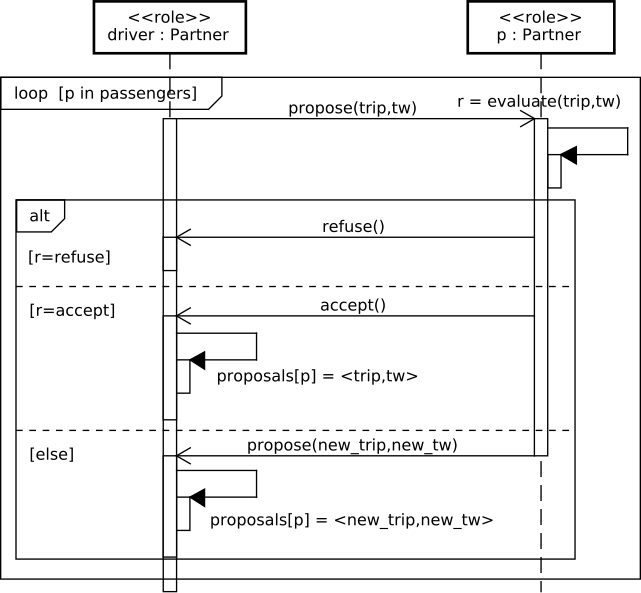
\includegraphics[width=.6\linewidth]{carpooling_negotiation_protocol1}
				\end{center}
			}
			\only<7>{
				\begin{center}
					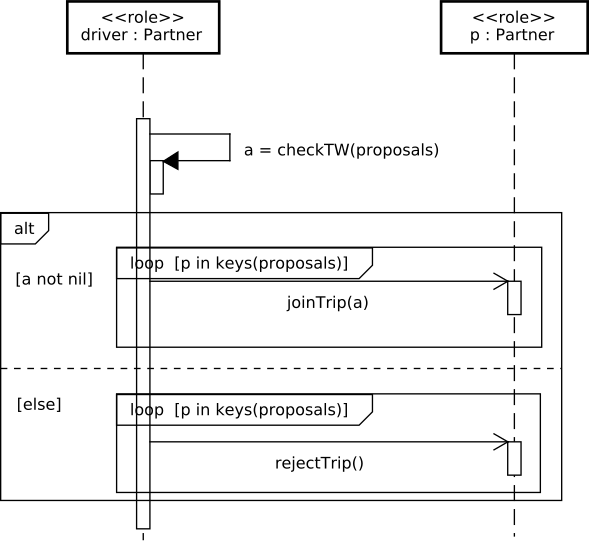
\includegraphics[width=.6\linewidth]{carpooling_negotiation_protocol2}
				\end{center}
			}
			\only<8>{
				\begin{block}{Time Preference Function}
					\begin{itemize}
					\item Each agent $A$ gives its preferences for the time of boarding/alighting:
						\[ f_A : \mathbb{R} \Rightarrow \mathbb{R} : t \mapsto f_A(t) \in [0,1] \]
					\end{itemize}
				\end{block}
				\vfill
				\begin{center}
					\zoombox{\includegraphicswtex[width=.4\linewidth]{carpooling_time_preference}}
				\end{center}
			}
			\only<9>{
				\smaller
				\begin{block}{Time Interval Suitability}
					\begin{itemize}
						\item Evaluate the suitability of times for boarding/alighting: 
						\[ \begin{cases}
						\int_{t}^{t+C} f_{A}(x)\cdot f_{B}(x) dx & \text{if } t \in [\max(\perp_{i_A},\perp_{i_B}),\min(\top_{i_A},\top_{i_B}) - C] \\
						0                                        & \text{otherwise} \\
						\end{cases} \]
					\end{itemize}
				\end{block}
				\begin{center}
					\zoombox{\includegraphicswtex[width=.75\linewidth]{carpooling_time_suitability}}
				\end{center}
			}
			\only<10>{
				\begin{columns}
					\begin{column}{.35\linewidth}
						\centering
						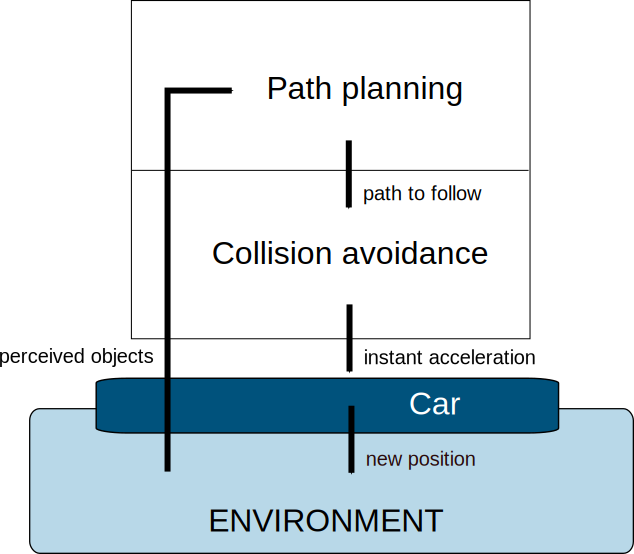
\includegraphics{carpooling_agent_layers}
						{\smaller\smaller\cite{GallandGaudDemangeKoukam2009_11}}
					\end{column}
					\begin{column}{.65\linewidth}
						\smaller
						\begin{block}{Path Planning}
						Based on the A* algorithm \cite{Dechter:1985:GBS:3828.3830,RoutePlanningAlgorithms2009} or D*-lite \cite{Koenig.Dstarlite.2005}
						\end{block}
						\begin{block}{Collision Avoidance}
							\begin{compactdescription}
							\item[Principle] compute the acceleration of the vehicle to avoid collisions with the other vehicles
							\item[Intelligent Driver Model] \cite{PhysRevE.62.1805}
							{\smaller
								\[acc = \begin{cases}
								- \dfrac{\left( v \Delta v \right)^2}{4b\Delta p^2} & \text{if the ahead object is far} \\
								- a \dfrac{\left( s + v w \right)^2}{\Delta p^2} & \text{if the ahead object is near} \\
								\end{cases}\]
							}
							\item[Free driving]
								{\smaller\[acc = a \left( 1 - \left(\frac{v}{v_c}\right)^4 \right)\]}
							\end{compactdescription}
						\end{block}
					\end{column}
				\end{columns}
			}
		\end{column}
	\end{columns}
\end{frame}

\end{graphicspathcontext}

\endinput

